\documentclass[aspectratio=169,11pt,hyperref={colorlinks=true}]{beamer}
\usetheme{boxes}
\setbeamertemplate{navigation symbols}{}
\definecolor{openstack}{RGB}{149,0,4}
\setbeamercolor{titlelike}{fg=openstack}
\setbeamercolor{structure}{fg=openstack}
\hypersetup{colorlinks,urlcolor=openstack}
\setbeamertemplate{footline}[frame number]
% Inserting graphics
\usepackage{graphicx}
% Side-by-side figures, etc
\usepackage{subfigure}
% Code snippits
\usepackage{listings}
\usepackage{lmodern}
% Color stuff
\usepackage{color}
\usepackage{amsmath}
\usepackage{tikz}
\newcommand\RBox[1]{%
  \tikz\node[draw,rounded corners,align=center,] {#1};%
}
\usepackage{hyperref}
%\usecolortheme{buzz}
%\usecolortheme{wolverine}
%\usetheme{Boadilla}
\usepackage[T1]{fontenc}

\definecolor{mygreen}{rgb}{0,0.6,0}
\definecolor{mygray}{rgb}{0.5,0.5,0.5}
\definecolor{mymauve}{rgb}{0.58,0,0.82}

\lstset{%
  backgroundcolor=\color{white},   % choose the background color; you must add \usepackage{color} or \usepackage{xcolor}
  breakatwhitespace=false,         % sets if automatic breaks should only happen at whitespace
  breaklines=true,                 % sets automatic line breaking
  captionpos=b,                    % sets the caption-position to bottom
  commentstyle=\color{openstack},  % comment style
  extendedchars=true,              % lets you use non-ASCII characters; for 8-bits encodings only, does not work with UTF-8
  keepspaces=true,                 % keeps spaces in text, useful for keeping indentation of code (possibly needs columns=flexible)
  keywordstyle=\color{blue},       % keyword style
%  otherkeywords={*,...},           % if you want to add more keywords to the set
  numbersep=5pt,                   % how far the line-numbers are from the code
  numberstyle=\tiny\color{mygray}, % the style that is used for the line-numbers
  rulecolor=\color{black},         % if not set, the frame-color may be changed on line-breaks within not-black text (e.g. comments (green here))
  showspaces=false,                % show spaces everywhere adding particular underscores; it overrides 'showstringspaces'
  showstringspaces=false,          % underline spaces within strings only
  showtabs=false,                  % show tabs within strings adding particular underscores
  stringstyle=\color{openstack},   % string literal style
}

\setbeamerfont{caption}{series=\normalfont,size=\fontsize{6}{8}}
\setbeamertemplate{caption}{\raggedright\insertcaption\par}

\setlength{\abovecaptionskip}{0pt}
\setlength{\floatsep}{0pt}

\author[Matthew Treinish & Matthew Oliver]{%
    \texorpdfstring{%
        \begin{columns}
            \column{.45\linewidth}
            \centering
            Matthew Treinish\\
            Developer Advocate - IBM\\
            \href{mailto:mtreinish@kortar.org}{mtreinish@kortar.org}\\
        \texttt{mtreinish on Freenode}
        \column{.45\linewidth}
            \centering
            Matthew Oliver\\
            Senior Software Engineer - SUSE\\
            \href{mailto:matt@oliver.net.au}{matt@oliver.net.au}\\
            \texttt{mattoliverau on Freenode}
        \end{columns}
        }
    {Matthew Treinish & Matthew Oliver}
}

\date{May 22, 2018}

\title[Keystone Federated Swift: Getting the Most Out of your Object Storage in a Federated Environment
\hspace{2em}\insertframenumber/\inserttotalframenumber]{Keystone Federated Swift: Getting the Most Out of your Object Storage in a Federated Environment}

\begin{document}

{%
\setbeamertemplate{background canvas}{
\includegraphics[width=\paperwidth,height=\paperheight]{background_title.png}}
\setbeamertemplate{footline}{}
\begin{frame}[noframenumbering]
    \setbeamercolor{titlelike}{fg=white}
    \setbeamercolor{structure}{fg=white}
    \setbeamercolor{normal text}{fg=white}
    \hypersetup{colorlinks,urlcolor=white}
    \setbeamercolor{author}{fg=white}
    \setbeamercolor{date}{fg=white}
    \setbeamercolor{background}{bg=openstack}
    \titlepage{}
    \centering
    \href{https://github.com/mtreinish/swift-keystone}{https://github.com/mtreinish/swift-keystone}
\end{frame}
}

\section{Keystone Federation}
\begin{frame}
    \frametitle{Why Keystone Federation?}
\end{frame}

\begin{frame}
    \frametitle{How it works}
\end{frame}

\begin{frame}
    \frametitle{Keystone with Swift}
\end{frame}

\section{Deployment Models}

\subsection{False Federation}
\begin{frame}
\frametitle{False Federation}
\centering
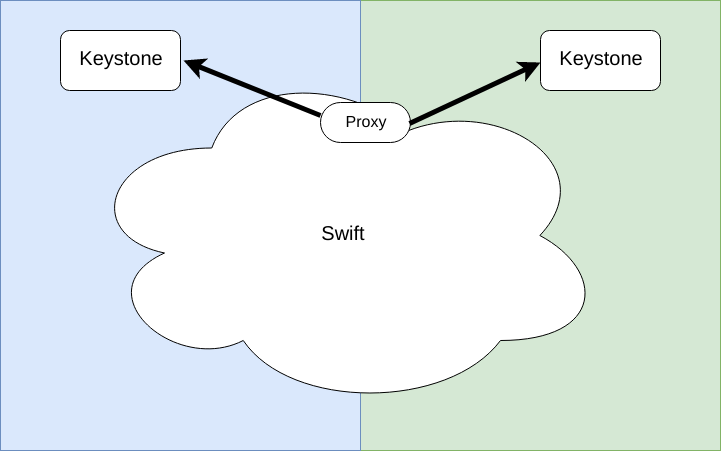
\includegraphics[width=.775\textwidth]{swift-federation-false.png}
\end{frame}

\subsection{Separate Swift Clusters}
\begin{frame}
\frametitle{Separate Swift Clusters}
\centering
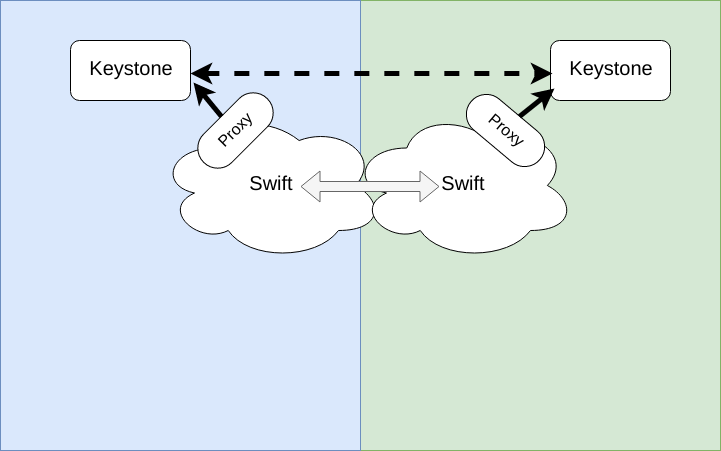
\includegraphics[width=.775\textwidth]{swift-federation-sep-container-sync.png}
\end{frame}

\subsection{Global Swift Cluster}
\begin{frame}
\frametitle{Global Swift Cluster}
\centering
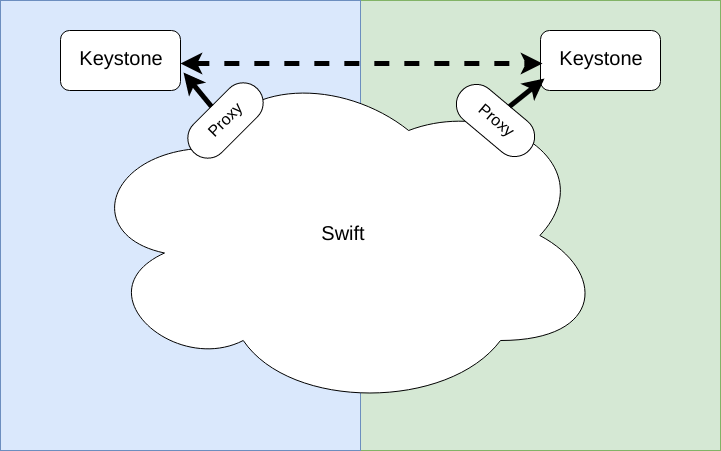
\includegraphics[width=.775\textwidth]{swift-federation-global.png}
\end{frame}

\section{More Information}
\begin{frame}
\frametitle{Where to get more information}
    \begin{itemize}
        \item Blog Post Series: \href{https://oliver.net.au/?p=335}{https://oliver.net.au/?p=335}
        \item openstack-dev ML: \href{mailto:openstack-dev@lists.openstack.org}{openstack-dev@lists.openstack.org}
        \item Details on Keystone Federation: \href{http://www.gazlene.net/demystifying-keystone-federation.html}{http://www.gazlene.net/demystifying-keystone-federation.html}
        \item These Slides: \href{https://github.com/mtreinish/swift-keystone}{https://github.com/mtreinish/swift-keystone}
   \end{itemize}
\end{frame}


\end{document}
